%!TEX root = ../thesis.tex

\chapter{Umsetzung}
\label{chap:coding}
In diesem Kapitel wird auf den Aufbau der Implementierung eingegangen. Zunächst ein allgemeiner Überblick über das Vorgehen. Dies wird im folgenden als Pipeline bezeichnet und wird im \prettyref{sec:pipeline} allgemein erkläutert.

Nachdem ein genereller Überblick über die einzelnen Bestandteile gegeben wurde wird auf die einzelnen Schritte der Pipeline genauer eingegangen.
Anfänglich werden einmalige Vorbereitungsschritte aufgeschlüsselt, hierzu gehört zu einem großen Teil die Kalibrierung der genutzten Kamera in \prettyref{sec:camera} und die Bestimmung der Charakteristika dieser. 

Darauf folgt in \prettyref{sec:board} die Kalibrierung und die Erkennung der Felder des Dartboardes. Es werden verschiedene getestete Ansätze erörtert und ihre Vor- und Nachteile dargestellt.

Des Weiteren werden die einzelnen Abschnitte der Pipeline näher beleuchtet und auf die Implementierung und das Vorgehen eingegangen. Dies umfasst von der Segmentierung der Dinge, die nicht zum Dartboard gehören in \prettyref{sec:segmentation}. Bis hin zur konkreten Bestimmung der erzielten Punktzahl in \prettyref{sec:score}. 
\todo{Umsetzung einteilen und implementieren}
       
\section{Pipeline Überblick}
\label{sec:pipeline}
Ein genereller Überblick über die Pipeline wird in Abbildung \prettyref{Fig:pipeline} gegeben. Zu erkennen ist, dass es zwei sich wiederholende Teile gibt. Als Verbindungsglied zwischen diesen steht der Contour Storage. Dieser speichert Informationen zu jedem aufgenommenen Bild. Auf den Storage, seine Funktionsweise und die weitere Verarbeitung wird in \prettyref{sec:foreground} eingegangen. 

Es wird ein einmalig, zu beginn ausgeführter Teil aufgerufen, der die Kalibrierung, der Kamera übernimmt. Diese gehört nur bedingt zur Pipeline hinzu. Die Kamera Kalibrierung muss für eine spezifische Kamera nur ein einziges mal ausgeführt werden, abgesehen von dem Fall, dass die Kamera eine Fokussierung besitzt. In diesem Fall muss dieser Schritt nach jedem Fokus Vorgang erneut ausgeführt werden. Auf die Kalibrierung der Kamera wird im einzelnen in \prettyref{sec:camera} eingegangen.

Ist die generelle Kalibrierung abgeschlossen, können die hieraus gewonnenen Informationen genutzt werden, um das Dartboard und dessen Felder zu segmentieren und unterscheiden zu können. Das Resultat dieser Kalibrierung ist eine Funktion, die eine Abbildung von einem Pixel zu einer spezifischen Punktzahl auf dem Dartboard darstellt. In \prettyref{sec:board} wird genauer beschrieben, welche Ansätze zu diesem Zweck verfolgt wurden und wie die letztendliche Umsetzung vorgenommen wurde.

Diese beiden Schritte können übersprungen werden, sofern das Setup sich nicht verändert hat, und die Kalibrierungen in einer Datei, als JSON, gespeichert wurden und erneut geladen werden können. 
\begin{figure}
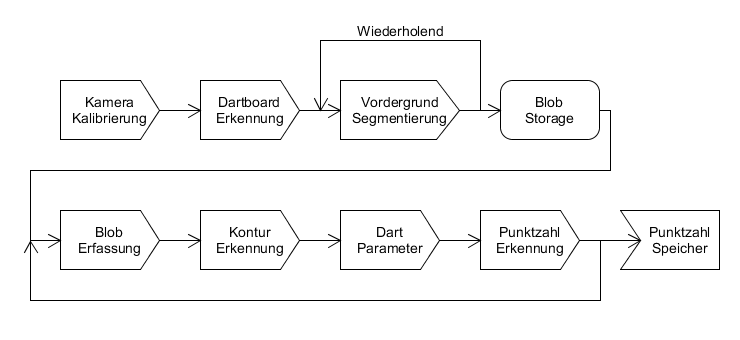
\includegraphics[width=\textwidth]{media/pipeline.png}\\
\caption{\textbf{Übersicht der einzelnen Schritte}}
\label{Fig:pipeline}
\end{figure}

Es werden zwei separate Threads gestartet. In der Abbildung ist der erste Thread grau markiert (Substrator) und der zweite türkis. Der Substractor dient dazu den Contour Storage mit Informationen zu füllen. In \prettyref{sec:substraction} wird das Vorgehen erläutert und welche Informationen bestimmt und gespeichert werden.
Der zweite Thread wird in mehrere Sub-Schritte unterteilt. 
Zunächst verwendet die Blob-Erfassung, mehr in \prettyref{sec:blob}, die Informationen im Storage um ein Bild zur weiteren Verarbeitung zu generieren. Die gewonnenen Informationen werden für die weitere Verarbeitung zu Kontur-Erkennung genutzt, nähere Beschreibung in \prettyref{sec:foreground}.

Abschließend werden die Dart-Parameter bestimmt und in der Punktzahl-Erkennung mithilfe der Bildpunkt-Punktzahl-Funktion in die erzielte Punktzahl überführt. Diese wird anschließend abgespeichert.


\section{Kamera Kalibrierung}
\label{sec:camera}
Im \prettyref{sec:camerageo} wurden bereits das Kamera Modell und die Parameter einer Kamera erläutert. So heißt es in \autocite[5]{Zhang2000} \textquote{Camera calibration is a necessary step in 3D computer vision in order to extract metric information from 2D images.} Nun gilt es eben diese Parameter zu bestimmen um genauere Daten aus den Bildern der Kamera zu erlangen. 

Diese Kalibrierung ist vorrangig dafür gedacht die intrinsischen Parameter der Kamera zu bestimmen. Die extrinsischen Parameter werden auf andere Art bestimmt, bzw. in einem anderen Schritt. Die Bestimmung der extrinsischen Parameter wird in \prettyref{sec:board} erläutert.

Es gibt mehrere verschiedene Möglichkeiten eine Kalibrierung der Kamera vorzunehmen. Diese sind: mit 3D-Objekten, mit 2D-Ebenen oder 1D-Linien. Dabei haben diese verschiedenen Varianten einen unterschiedlich hohen Aufwand, Genauigkeit und Komplexität in der Berechnung. 

So muss für jede dieser Varianten bestimmte Features und deren Position bekannt sein. Dies ist bei einem 3D-Objekt schwieriger zu bestimmen, als bei einer Ebene. Daher wurde der Einfachheit halber auf die Ebene zurückgegriffen. 
\begin{figure}
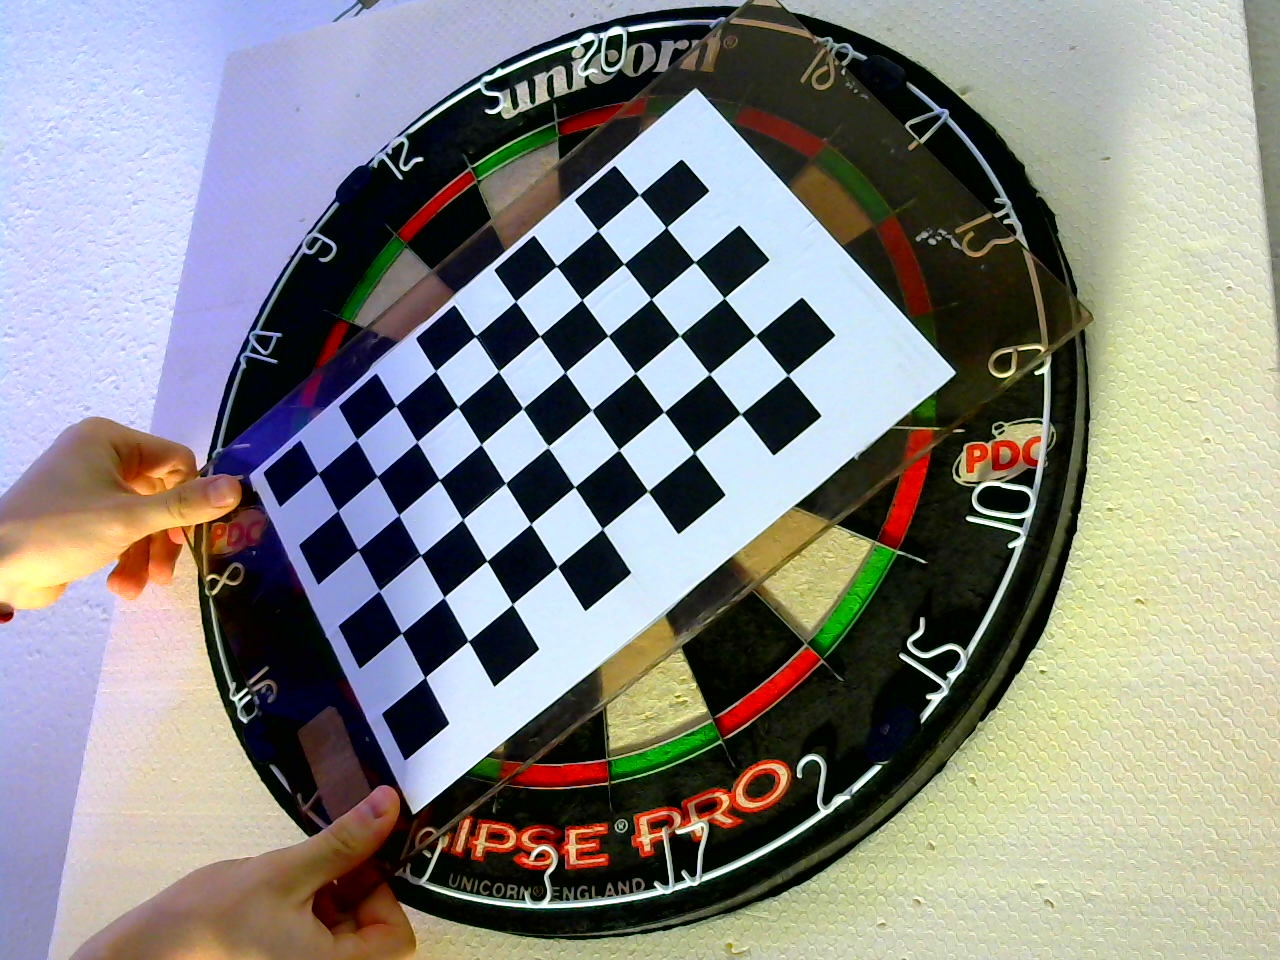
\includegraphics[width=\textwidth]{media/calibraw1.jpg}\\
\caption{\textbf{Eines der zur Kalibrierung genutzten Bilder}}
\label{Fig:calibplane}
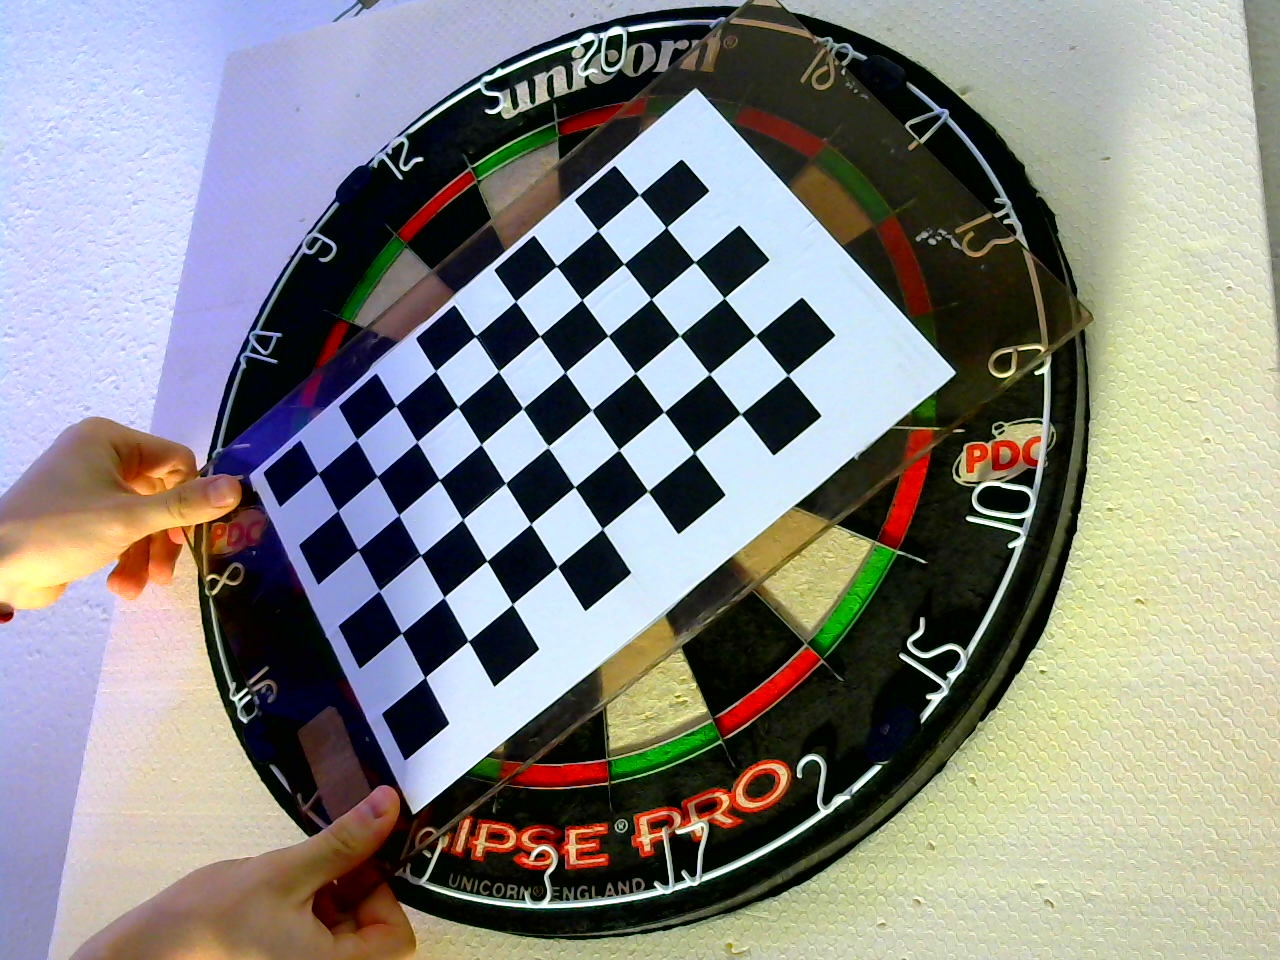
\includegraphics[width=\textwidth]{media/calibraw1.jpg}\\
\caption{\textbf{Erkannte Feature Punkte/Schnittpunkte}}
\label{Fig:calibplanefeature}
\end{figure}
In Abbildung \prettyref{Fig:calibplane} ist eines der Bilder zu sehen, mit denen die zum Test der Implementierung genutzten Kamera kalibriert wurde. Dies ist ein Muster von $9x6$ Schnittpunkten. In Abbildung \prettyref{Fig:calibplanefeature} \todo{korrektes Bild einfügen} sind die erkannten Feature-Punkte eingezeichnet. Für dieses Schachbrettmuster ist der Abstand der einzelnen Schnittpunkte durch ausmessen bekannt und mit $26mm$ Abstand entlang der Graden voneinander gegeben. 

Wie bereits beschrieben wird OpenCV \prettyref{sec:opencv} zur Implementierung genutzt. OpenCV bietet einige Funktionen um die Kamera Kalibrierung durchzuführen. Die Dokumentation von OpenCV3 \autocite{Opencv3Camera2016} zeigt die dafür zur Verfügung gestellten Funktionen. 
\begin{lstlisting}[frame=single]
ret, corners = findChessboardCorners(image, patternSize) 
corners2 = cornerSubPix(image, corners, winSize, zeroZone,\\
               criteria) 
ret, mtx, dist, rvecs, tvecs = calibrateCamera(\\
               objectPoints, imagePoints, imageSize,\\
               cameraMatrix, distCoeffs[, rvecs[,\\
               tvecs[, flags[, criteria]]]]) 
newcameramtx, roi = getOptimalNewCameraMatrix(mtx, dist,\\
               imageSize, alpha , newimageSize)
\end{lstlisting}
So wird \textit{findChessboardCorners} verwendet um die Schnittpunkte im Schachbrettmuster zu erkennen und die dazugehörigen Koordinaten zu identifizieren. Hierzu wird eines der Bilder mit dem Schachbrettmuster in ein Graustufenbild gewandelt und der Funktion übergeben, zusätzlich wird die Größe des Schachbrettmusters übergeben $(9,6)$. Dies liefert zum einen den Erfolg der Funktion als Boolean zurück und zum anderen die Bildkoordinaten der gefundenen Schnittpunkte. 
Die gefundenen Koordinaten sind allerdings nur approximierte Werte, daher ist es empfehlenswert \textit{cornerSubPix} auf demselben Bild mit den bereits ermittelten Schnittpunkten aufzurufen. Diese dient der genaueren Bestimmung der Bildkoordinaten, um eine bessere Genauigkeit zu erreichen. Die Funktion gibt die neuen Koordinaten der Schnittpunkte zurück. 

Um die Parameter der Kamera zu errechnen werden die Bildpunkte, der Schachbrettschnittpunkte und die zugehörigen Objektpunkte benötigt. Die Objektpunkte sind in diesem Fall die Punkte auf dem Schachbrett. Es wird davon ausgegangen, dass sich die Punkte alle auf einer Ebene befinden \textit{z=0}. Die Objektpunkte sehen in etwa wie folgt aus: $[[0,0,0], [26,0,0],...,[0,26,0],[0,52,0],...,[234,156,0]]$

Da es einer Ungenauigkeit, durch Rauschen und andere Fehler kommen kann wird nicht nur ein Bild zur Kalibrierung genutzt, sondern mehrere. Um eine der Linien entlang des Schachbrettmusters zu bestimmen reichen in der Theorie zwei Punkte. Aus bereits genannten Gründen werden allerdings auch hier mehrere Punkte verwendet. Zudem wird kein quadratisches Schachbrett genutzt, da so die Orientierung des Musters erkannt werden kann. 
Der in OpenCV verwendete Algorithmus basiert auf der Arbeit von Zhengyou Zhang. In "`Emerging Topics in Computer Vision"' \autocite{Medioni:2004:ETC:993884} empfiehlt dieser: \textquote{(...), we recommend 4 or 5 different orientations for better quality.} \autocite[24]{Zhang2000}.

So werden zu mehreren Bildern, mit unterschiedlicher Orientierung des Schachbrettes zur Kamera, die Bildpunkte bestimmt und gespeichert. Diese werden anschließend gesammelt an die Funktion \textit{calibrateCamera} übergeben. \textit{criteria} enthält Informationen für den Berechnungsalgorithmus, wie zum Beispiel die Distanz zwischen zwei Schnittpunkten. Die weiteren Parameter der Funktion sind optional und dienen der genaueren Berechnung.
Die Funktion gibt fünf Dinge zurück: \textit{ret} ist ein Boolean, ob die Berechnung erfolgreich war, \textit{mtx} die Kameramatrix, die die intrinsischen Parameter der Kamera enthält, \textit{dist} die Verzerrungsparameter, \textit{rvecs} ein Rotationsvektor, der die Rotation zwischen Kamera und Schachbrettmuster wiedergibt und zuletzt \textit{tvecs} ein Translationsvektor, der die Translation zwischen Kamera und Schachbrettmuster wiedergibt. Dabei sind Rotations- und Translationsvektor nicht weiter von Interesse, da diese nicht die Relation zum Dartboard wiedergeben. Wie die hierfür nötigen Vektoren bestimmt werden wird in \prettyref{sec:board} erläutert. Ein Beispiel für eine Matrix mit der genutzten Kamera sieht wie folgt aus:
$A= 
\begin{bmatrix} 
1416.55 & 0.0 & 687.84 \\
0.0 & 1416.51 & 476.39 \\
0.0 & 0.0 & 1.0\end{bmatrix}$.

Damit der Kalibrierungsvorgang nicht zu jedem Start der Software durchgeführt werden muss, werden die gewonnenen Parameter als JSON-String in eine Datei geschrieben. Zur nächsten Ausführung der Software kann dieser wieder geladen werden. 


\section{Erkennung des Dartboards}
\label{sec:board}
Stage 1 Board finden:
     mehrere Ansätze
     Blobs des boardes erkennen
     Felder Kanten erkennen
     Board Kalibrieren als Erweiterung der Kamera Kalibrierung
        
        Dartboard Koordinaten bestimmen im Verhältnis zur Kamera.
       Eigentliche Kalibrierung via klicken,
       wie viele Punkte sind nötig


\section{Extraktion des Vordergrundes}
\label{sec:substraction}
Stage 3 Vordergrund von Hintergrund trennen
Foreground detection naiver Ansatz und Algorithmen
Parameter Erklärung
Vereinfachung und Annahmen
Aufgetretene Problematik

\section{Blob Erfassung}
\label{sec:blob}


\section{Verarbeitung der Vordergrundinformationen}
\label{sec:foreground}
Stage 4 Im Extrahierten Vordergrund entscheiden was Pfeil ist
\section{Punktzahlbestimmung}
\label{sec:score}
Stage 5 Parameter vom Pfeil bestimmen(Spitzen)
